%%%%%%%%%%%%%%%%%%%%%%%%%%%%%%%%%%%%%%%%%%%%%%%%%%%%%%%%%%%%%%%%%%%%%%%%%%%%%%%%
% Anonymous ICRA 2027 draft.
% Red \todo{...} / \tbd marks are placeholders for results not yet produced.
% Search for "todo" before submission. Layout is tuned at the very end.
%%%%%%%%%%%%%%%%%%%%%%%%%%%%%%%%%%%%%%%%%%%%%%%%%%%%%%%%%%%%%%%%%%%%%%%%%%%%%%%%
\documentclass[letterpaper, 10pt, conference]{ieeeconf}
\IEEEoverridecommandlockouts
\overrideIEEEmargins
\usepackage{amsmath,amssymb,booktabs,multirow,graphicx,xcolor,cite,url,microtype,newtxtext,newtxmath,algorithm,algorithmic,dblfloatfix,placeins,flushend}
\newcommand{\vect}[1]{\mathbf{#1}}
\newcommand{\todo}[1]{\textcolor{red}{[TODO: #1]}}
\newcommand{\tbd}{\textcolor{red}{TODO}}
\setcounter{topnumber}{3}
\setcounter{dbltopnumber}{3}
\setcounter{totalnumber}{4}
\renewcommand{\topfraction}{0.9}
\renewcommand{\dbltopfraction}{0.9}
\renewcommand{\textfraction}{0.05}
\renewcommand{\floatpagefraction}{0.85}
\renewcommand{\dblfloatpagefraction}{0.85}

\title{\LARGE \bf DARE: Differential Adversarial Reward Equalization for Humanoid Motion Imitation}
\author{Anonymous Authors}

\begin{document}
\maketitle
\thispagestyle{empty}
\pagestyle{empty}

\begin{abstract}
Physics-based humanoid motion imitation requires simultaneously tracking multiple objectives, including root motion, body pose, and velocities. Existing methods often rely on handcrafted reward terms with manually tuned weights and scales, which can require substantial adjustment across different motions. We propose DARE (Differential Adversarial Reward Equalization), an adversarially learned reward method based on the differential between the reference motion and the policy state. DARE represents perfect tracking as a zero differential and learns a unified tracking reward from policy-generated residuals, while controlling discriminator sensitivity and automatically calibrating its output scale to support a consistent reward configuration across motions. We evaluate DARE on multiple humanoid skills with diverse dynamics and contact patterns. The results show that DARE achieves stable and accurate motion tracking without motion-specific reward tuning.
\end{abstract}

\section{Introduction}
Physics-based humanoid motion imitation requires the controller to
reproduce a prescribed reference motion under dynamic constraints,
actuator limits, and complex contact conditions. Whether an imitation
succeeds is not a single geometric question. The root must translate and
turn as the reference does, the articulated body must maintain consistent
poses, joint and root velocities must stay synchronized with the reference
motion, and contacts must occur at the right moments. Because these
objectives have different physical units, numerical ranges, and dynamical
characteristics, and are coupled through the robot dynamics, motion
imitation is inherently a multi-objective control problem.

Traditional methods transform several tracking errors separately and
combine them into a scalar reward through manually chosen weights and
scales. These coefficients determine both the relative importance and the
numerical response of the tracking objectives. Because typical errors and
dynamical difficulty change with the motion, a coefficient set that serves
one skill need not serve another; in practice, reward design is often
re-tuned whenever the reference motion changes.

Adversarial imitation offers a way to reduce manual reward design.
Instead of declaring in advance how many meters of root-position error
are worth how many radians of rotation error, a discriminator learns a
unified imitation signal directly from data. AMP and related methods
learn rewards that describe motion style and plausibility by
discriminating whether short state transitions come from the reference
distribution \cite{peng2021amp}. For motion tracking that must strictly
follow a synchronized reference trajectory, ADD further feeds the
reference--policy state differential to the discriminator and asks
whether it is close to the ideal zero differential \cite{zhang2025add}.
The aggregation among tracking objectives can then be learned by the
discriminator instead of specifying component-wise weights and scales by
hand.

Differential adversarial rewards, however, still face an important issue.
Their ideal sample is always a single point, the zero differential.
Without a suitable constraint, the discriminator easily becomes too
sharp: it assigns a high score to the origin and compresses the many
nonzero residuals produced by the policy into a nearby low-score region.
Even if classification succeeds, the discriminator may not provide an
effective continuous learning signal for the policy. Existing methods
constrain the discriminator through regularization, but one regularizer
simultaneously affects two distinct properties. On the one hand, it
controls the discriminator's local sensitivity, that is, how fast the
score changes with the input residual. On the other hand, it also affects
the numerical range in which the final scores live, and this range in turn
determines whether the policy reward operates in an effective interval.
As the residual distribution changes across motions, the same
regularization setting can correspond to different sensitivities and
different score scales, producing motion-dependent effective
regularization requirements.

The core idea of DARE is to treat these two issues separately rather than
control them with one motion-dependent coefficient. First, DARE applies
spectral normalization to every linear layer of the differential
discriminator, directly bounding the maximum amplification of residual
variations. Second, after residual normalization is fixed, DARE measures
the score separation between the unique zero-error anchor and
representative policy residuals and rescales the discriminator once in
closed form. The geometry constraint and reward operating scale are thus
specified independently.

Constraining the critic's sensitivity alone does not resolve the score
scale. A Lipschitz bound controls how rapidly the score may change, but
not the numerical range actually used by the trained critic. DARE
therefore measures the anchor-to-typical-residual score gap once after
normalization stabilizes and uses a closed-form global rescaling tied to
the response range of the reward transform. All motions use exactly the
same calibration rule; the only quantity that changes across motions is
the residual statistic measured automatically from the training data.
The critic's geometry and score scale thus no longer depend on the same
hand-tuned parameter.

The main contributions are threefold. First, we identify that the
regularizer in existing differential adversarial rewards simultaneously
affects the critic's local geometry and its score scale, and that this
coupling can make different motions require different effective
regularization settings. Second, we propose DARE, which constrains
discriminator sensitivity through layer-wise spectral normalization and
sets the score scale automatically through one-shot anchor calibration,
removing the need for a motion-specific gradient-penalty coefficient.
Third, we evaluate one shared DARE configuration on six skills with
different durations, contact patterns, and dynamical characteristics.

\section{Related Work}
\textbf{Physics-based motion tracking and learned imitation objectives.}
DeepMimic combines pose, velocity, root, and end-effector tracking terms
for physics-based skills \cite{peng2018deepmimic}; subsequent work
improves scalability and motion coverage through architectures,
representations, and data \cite{luo2023phc,tessler2023maskedmimic}.
Adversarial imitation provides a learned alternative to a manually
written reward: GAIL matches expert and policy occupancies
\cite{ho2016gail}, while AMP learns a motion prior by discriminating
short state transitions \cite{peng2021amp}. ADD addresses
reference-conditioned tracking by presenting the reference--policy
differential to an adversarial discriminator and learning a nonlinear
aggregation of tracking objectives without component-wise reward weights
\cite{zhang2025add}.

\textbf{Multi-objective learning and objective aggregation.} Competing
objectives are commonly combined by weighted scalarization, Pareto
optimization, or adaptive loss weighting
\cite{sener2018multitask,kendall2018multi}. These approaches differ in
whether preferences are specified explicitly or adapted from objective
statistics. In differential adversarial tracking, the discriminator
instead learns this aggregation from the joint residual distribution.

\textbf{Regularization of adversarial critics.} Adversarial critics are
regularized with gradient penalties or spectral normalization to control
sensitivity and improve optimization
\cite{gulrajani2017improved,miyato2018spectral}. Gradient penalties
constrain sampled input derivatives, whereas spectral normalization
bounds the gain of individual network maps by construction. For
non-Wasserstein adversarial losses, the numerical score range also
determines the operating regime of the loss and its reward transform
\cite{karras2020ada}. Geometry and score calibration are therefore
related but distinct considerations when a critic supplies the learning
signal.

\section{Background}
\subsection{Reference-Conditioned Motion Tracking}
In reference-conditioned humanoid motion imitation, the controller must
keep the executed motion continuously aligned with a time-synchronized
reference trajectory. Let $s_t$ and $\hat{s}_t$ denote the current state
and the reference state at time $t$. Tracking quality is jointly measured
by several physical quantities, including root position and orientation,
articulated body pose, and motion velocities. Let $\phi_i(s_t)$ extract
the $i$-th tracking quantity from the current state and let
$\phi_i(\hat{s}_t)$ denote its reference counterpart. These quantities
may have different dimensions and physical units---positions are measured
in meters, while rotations and velocities have their own representations.

\subsection{Handcrafted Objective Scalarization}
Traditional methods first compress each tracking error into a scalar.
For tracked quantity $i$, the scalar tracking error at time $t$ is the
Euclidean distance
$e_{i,t}=\|\phi_i(\hat{s}_t)-\phi_i(s_t)\|_2$.

A representative handcrafted scalarization is
\begin{equation}
r_t^{\mathrm{hand}}=\sum_i w_i\exp\!\left(-\alpha_i e_{i,t}^2\right),
\label{eq:hand}
\end{equation}
where $w_i$ and $\alpha_i$ set the relative importance and numerical
scale of each tracking quantity. DeepMimic is a representative instance
of this class: its
tracking terms use weights and error scales specified before training and
held fixed throughout \cite{peng2018deepmimic}. This is a fixed
scalarization of the tracking objectives: the trade-off among errors is
fixed through constant coefficients chosen before training starts.
Because typical error magnitudes and dynamical characteristics differ
across motions, one coefficient set need not serve all motions. Learned
scalarization instead leaves the trade-off unspecified in advance and
learns the aggregation among objectives from the error distribution that
actually occurs during training.

\subsection{Differential Adversarial Objectives}
\label{sec:learned}

Differential adversarial learning provides such a learned aggregation
\cite{zhang2025add}. Consider $n$ non-negative objective losses
$l^1,\ldots,l^n$ collected into a differential vector
$\Delta=(l^1,\ldots,l^n)$, where each entry records the gap between the
current solution and the ideal on one objective. When all objectives are
simultaneously ideal, $\Delta=0$. A discriminator is trained to assign a
high score to the ideal zero differential and lower scores to the nonzero
differentials produced by the current policy. Because it receives all
objective differentials jointly, the discriminator can learn a nonlinear
aggregation of the objectives without fixed per-objective weights. Its
sensitivity to individual objectives may vary across the residual space
and throughout training, allowing the learned aggregation to adapt to the
differential distribution encountered during optimization.

In synchronized motion tracking, the differential can be formed directly
from the feature residual between the current and reference states rather
than from one scalar loss per objective. Perfect tracking again corresponds
to the unique zero differential, while nonzero differentials preserve the
magnitude, direction, and correlations of the tracking errors. The
discriminator score can therefore be used to construct a policy reward
that increases as the current differential is judged more consistent with
perfect tracking.

\begin{figure*}[t]
\centering
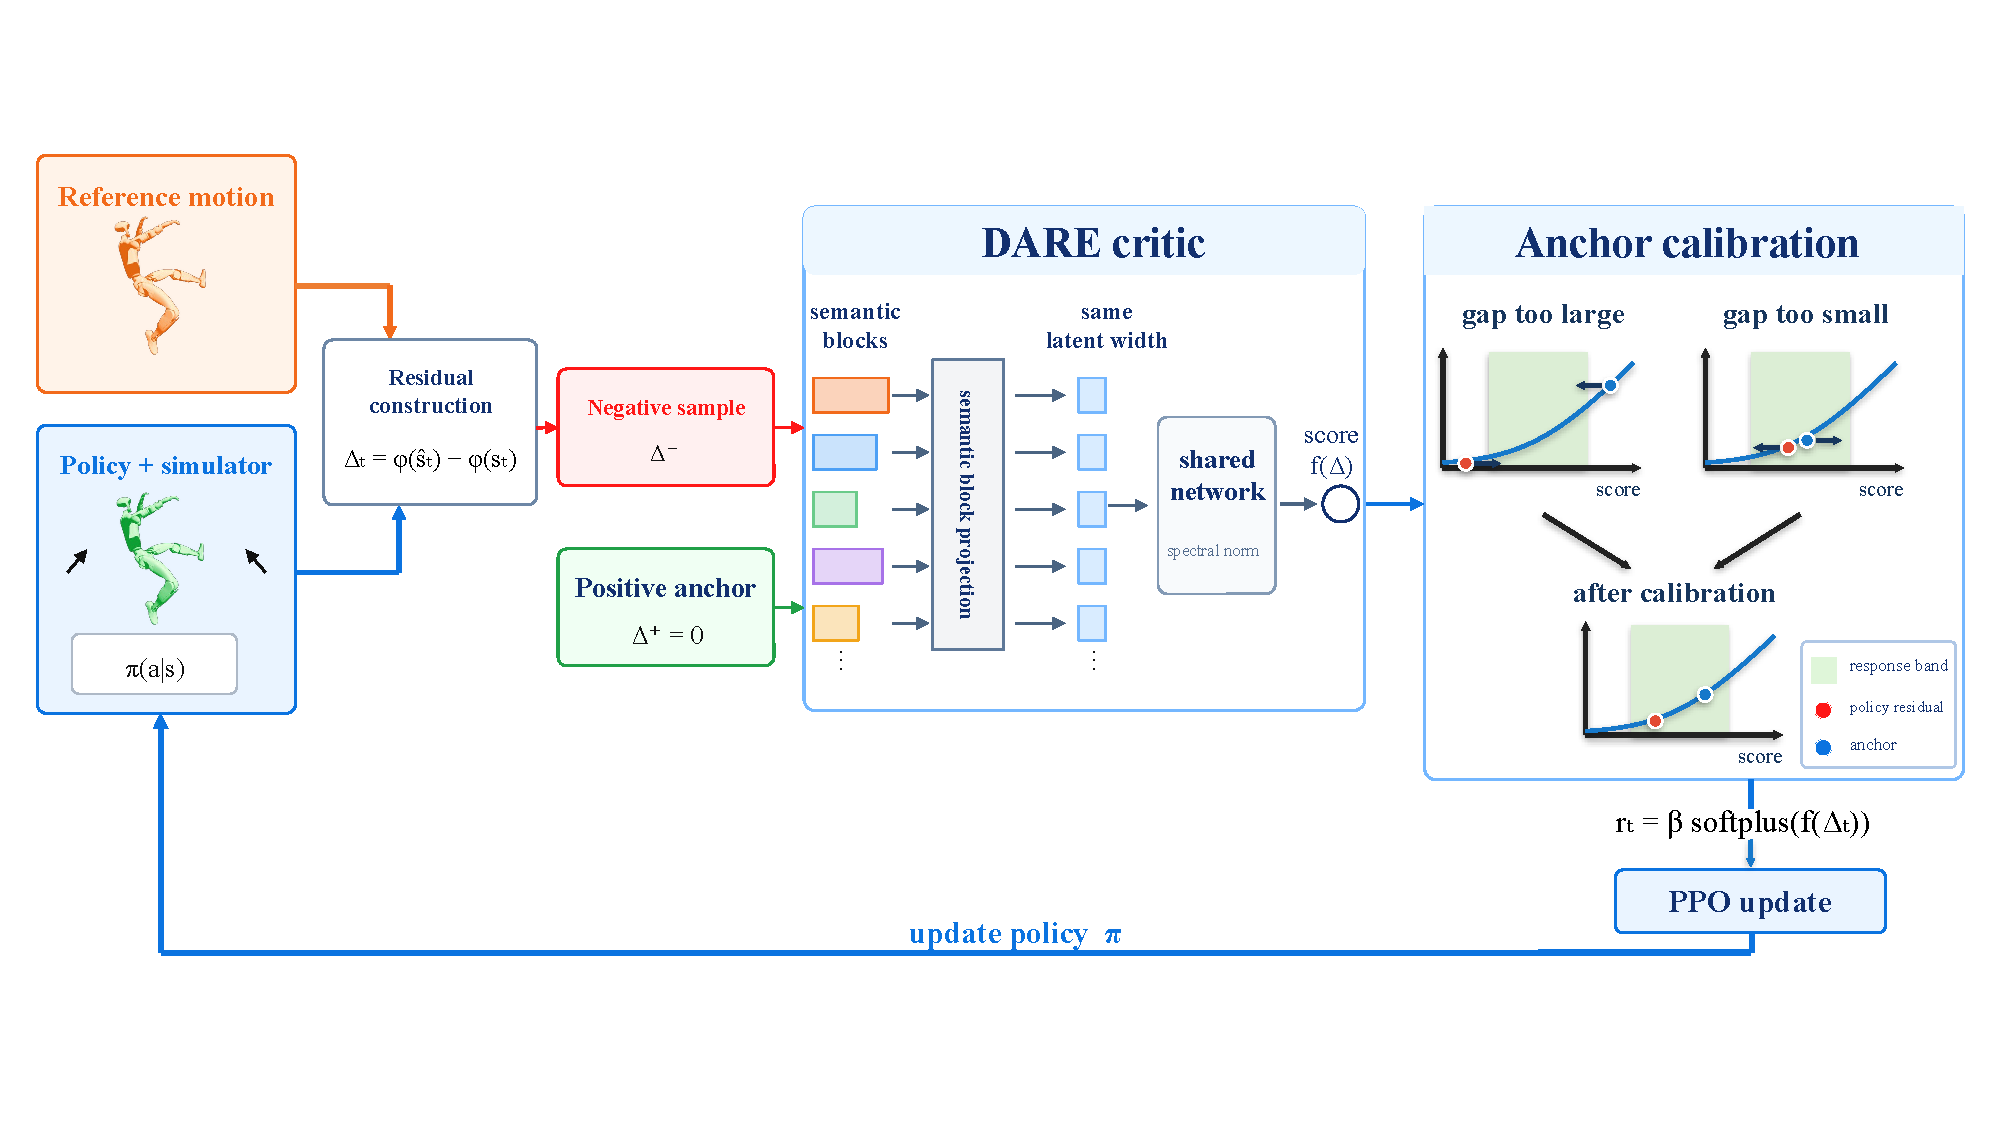
\includegraphics[width=0.88\textwidth,trim=0 64 0 0,clip]{figures/pipeline.pdf}
\caption{DARE training loop. The synchronized reference and simulated
state form the policy residual. The residual and zero anchor train the
equalized discriminator; one-shot anchor calibration rescales its logit,
and the resulting softplus reward drives the PPO update.}
\label{fig:pipeline}
\end{figure*}

\section{DARE: Differential Adversarial Reward Equalization}
\label{sec:dare}

\subsection{Learned Differential Reward}
\label{sec:reward}

Motion tracking involves multiple objectives with different physical meanings.
Rather than compressing them into separately weighted scalar terms, DARE
forms one full reference--policy residual. Let
\(\phi(s_t)\in\mathbb{R}^{d}\) collect the tracked quantities and let
\(\nu\in\mathbb{R}^{d}\) contain their per-coordinate mean-absolute scales,
estimated during early training and fixed after the first \(10^{8}\) samples.
The normalized differential is
\(\Delta_t=\delta_t\oslash\nu\), where
\(\delta_t=\phi(\hat{s}_t)-\phi(s_t)\), and perfect tracking is represented
by \(\Delta^{+}=0\). Here \(\oslash\) denotes element-wise division.
Because normalization only rescales coordinates and introduces no offset,
perfect tracking remains the unique zero differential. Rotational quantities
use a tangent--normal representation so that all tracked residuals are
represented in consistent Euclidean coordinates.

The full differential retains coordinate-wise error magnitudes, directions,
and correlations. Two states can therefore have the same aggregate distance
while differing in which tracked quantities deviate from the reference.
Let \(q_\pi\) denote the distribution of differentials induced by policy
\(\pi\). During training, recently generated policy differentials are stored
in a replay buffer and reused as negative samples for discriminator updates.

DARE maps the full differential to a scalar discriminator logit,
\(f_\theta:\mathbb{R}^{d}\rightarrow\mathbb{R}\). A larger
\(f_\theta(\Delta)\) indicates that the differential is judged more
consistent with perfect tracking. We introduce a global logit scale
\(\kappa>0\), initialized to \(1\) and determined automatically once by the
anchor calibration described in Sec.~\ref{sec:calibration}. The scaled logit
used for discriminator training and policy reward is therefore
\(\kappa f_\theta(\Delta)\).

Perfect tracking defines the positive differential \(\Delta^+=0\), while
differentials induced by policy \(\pi\) form the negative class, with
\(\Delta^-\sim q_\pi\). The discriminator is trained with the balanced
binary logistic loss
\begin{align}
\mathcal{L}_{\mathrm{DARE}}(\theta)
&=
\frac{1}{2}\,
\operatorname{softplus}
\!\left[-\kappa f_\theta(\Delta^{+})\right]
\notag\\
&\quad+
\frac{1}{2}\,
\mathbb{E}_{\Delta^{-}\sim q_\pi}
\operatorname{softplus}
\!\left[\kappa f_\theta(\Delta^{-})\right].
\label{eq:dare_loss}
\end{align}

The first term encourages a large logit for the zero differential, while
the second encourages lower logits for policy-induced residuals. Because
the discriminator receives all residual coordinates jointly, it learns
from data how the different tracking errors should contribute to a single
score.

The policy reward is constructed from the same scaled logit:
\begin{equation}
r_t^{\mathrm{DARE}}
=
\operatorname{softplus}
\!\left[\kappa f_\theta(\Delta_t)\right].
\label{eq:reward}
\end{equation}
Since softplus is strictly increasing, a larger discriminator logit produces
a larger policy reward. The learned reward therefore encourages the policy
toward residuals that the discriminator judges more consistent with perfect
tracking, while jointly accounting for root motion, body pose, and
velocities.


\subsection{Equalized Discriminator: Sensitivity Constrained by Construction}
\label{sec:critic}

The differential discriminator must not only distinguish perfect tracking
from policy-induced residuals, but also provide the policy with a continuous
reward signal that reflects differences in tracking quality. Its sensitivity
to the tracking differential therefore needs to be controlled. Since perfect
tracking always corresponds to the unique zero differential
\(\Delta^{+}=0\), excessive sensitivity near the origin can cause the
discriminator logit to decrease sharply even for a small deviation from
zero. In this case, although the discriminator may still separate positive
and negative samples, nonzero residuals of different quality can be compressed
into a similar low-score region, weakening the ability of the reward to
distinguish tracking quality.

A common approach is to introduce a gradient penalty during discriminator
training to limit excessive input sensitivity~\cite{zhang2025add}. However,
this introduces an additional regularization strength: if the constraint is
too weak, the discriminator may remain overly sensitive; if it is too strong,
the discriminator may become overly smooth and lose its ability to distinguish
different residuals. DARE instead constrains the maximum response of the
discriminator directly through its network structure, without introducing an
additional balancing coefficient.

The normalized full tracking differential
\(\Delta\in\mathbb{R}^{d}\) is fed directly into the discriminator. Let the
network contain \(L\) affine layers, with weight matrix \(W_\ell\) and bias
\(b_\ell\) at layer \(\ell\). DARE applies spectral normalization to every
weight matrix,
\[
\bar W_\ell
=
\frac{W_\ell}{\sigma_{\max}(W_\ell)}.
\]
Here, \(\sigma_{\max}(W_\ell)\) is the largest singular value of
\(W_\ell\), defined as
\[
\sigma_{\max}(W_\ell)
=
\max_{v\neq0}
\frac{\|W_\ell v\|_2}{\|v\|_2}.
\]
It therefore gives the maximum factor by which the linear map can amplify
an input variation. Consequently, for any vector \(v\),
\[
\|W_\ell v\|_2
\le
\sigma_{\max}(W_\ell)\|v\|_2.
\]
After spectral normalization,
\(\sigma_{\max}(\bar W_\ell)=1\). The network uses ReLU as the activation
function \(\rho\), which is also \(1\)-Lipschitz and therefore does not
increase the Euclidean distance between two inputs.

Consider an arbitrary hidden layer \(\ell\), and let \(x\) and \(x'\) denote
two inputs to this layer. Its outputs satisfy
\begin{align}
&
\left\|
\rho(\bar W_\ell x+b_\ell)
-
\rho(\bar W_\ell x'+b_\ell)
\right\|_2
\notag\\
&\qquad\le
\left\|
\bar W_\ell(x-x')
\right\|_2
\notag\\
&\qquad\le
\sigma_{\max}(\bar W_\ell)
\|x-x'\|_2
=
\|x-x'\|_2 .
\label{eq:layer_bound}
\end{align}

The first inequality follows from the \(1\)-Lipschitz property of ReLU;
the common bias \(b_\ell\) cancels when the two pre-activations are compared.
The second follows directly from the largest-singular-value bound above,
and the final equality follows from
\(\sigma_{\max}(\bar W_\ell)=1\). Thus, every hidden layer is
non-expansive. The final affine output layer obeys the same bound without
the ReLU activation. Applying this relation successively through all layers
therefore gives
\begin{equation}
\left|
f_\theta(\Delta)-f_\theta(\Delta')
\right|
\le
\left\|
\Delta-\Delta'
\right\|_2 .
\label{eq:pairwise_bound}
\end{equation}

Thus, a small change in the tracking differential cannot be arbitrarily
amplified into a large change in the discriminator logit; its maximum
sensitivity is directly constrained by the network structure.

Since perfect tracking corresponds to the zero differential
\(\Delta^{+}=0\), setting \(\Delta'=0\) in
Eq.~\eqref{eq:pairwise_bound} gives
\begin{equation}
\left|
f_\theta(\Delta)-f_\theta(0)
\right|
\le
\|\Delta\|_2 .
\label{eq:anchor_bound}
\end{equation}

Therefore, when the tracking differential is close to the perfect-tracking
anchor, the discriminator logit cannot change arbitrarily rapidly relative
to its value at zero residual. DARE thereby constrains the maximum response
of the discriminator to tracking residuals through layer-wise spectral
normalization.


\subsection{Anchor Calibration: Closed-Form Output Scale}
\label{sec:calibration}

Spectral normalization constrains how rapidly the raw discriminator logit
\(f_\theta(\Delta)\) can change with the tracking differential, but it does
not determine the global numerical scale of the logit used by the reward.
DARE controls this remaining degree of freedom through the global scale
\(\kappa\).

For a scalar logit \(z\), the slope of the softplus reward is
\begin{equation}
\frac{d}{dz}\operatorname{softplus}(z)
=
\sigma(z).
\label{eq:reward_slope}
\end{equation}
When \(z\) is sufficiently negative, \(\sigma(z)\) is close to zero, so
changes in the logit produce only small reward differences. Around
\(z=0\), the reward becomes more responsive, and as \(z\) increases the
slope approaches one. DARE therefore uses the interval over which the
softplus slope increases from \(0.2\) to \(0.8\) as its target response
region. Its width is
\begin{equation}
w
=
\sigma^{-1}(0.8)
-
\sigma^{-1}(0.2)
=
\ln 16
\approx 2.77 .
\label{eq:response_width}
\end{equation}

The target width \(w\) specifies the desired separation in scaled-logit
space. To determine the corresponding scale automatically, DARE measures
the separation produced by the discriminator itself. At calibration time
\(t_f\), let
\begin{equation}
M_f
=
f_\theta(0)
-
\frac{1}{2}
\left[
\mathbb{E}_{\Delta\sim q_{\mathrm{cur}}}
f_\theta(\Delta)
+
\mathbb{E}_{\Delta\sim q_{\mathrm{rep}}}
f_\theta(\Delta)
\right]
\Bigg|_{t=t_f},
\label{eq:anchor_gap}
\end{equation}
where \(q_{\mathrm{cur}}\) and \(q_{\mathrm{rep}}\) denote the residual
differential distributions from the current rollout and replay buffer,
respectively. Thus, \(M_f\) is the raw-logit separation between the
zero-differential anchor and the policy residuals observed at calibration.

DARE then sets the global logit scale in closed form:
\begin{equation}
\kappa
=
\frac{w}{M_f}.
\label{eq:kappa}
\end{equation}
The measured separation is therefore rescaled from \(M_f\) to
\(\kappa M_f=w\). If \(M_f>w\), then \(\kappa<1\) and an overly wide
separation is compressed; if \(M_f<w\), then \(\kappa>1\) and an overly
narrow separation is enlarged. Since the same positive factor multiplies
every discriminator logit, this operation preserves their ordering and only
changes the global output scale.

Calibration is performed once after the input normalization is fixed.
Before calibration, \(\kappa=1\). After Eq.~\eqref{eq:kappa} is evaluated,
\(\kappa\) is kept fixed and the scaled logit
\(\kappa f_\theta(\Delta)\) is used consistently in both discriminator
optimization and policy reward computation. Spectral normalization therefore
controls the sensitivity of the raw discriminator mapping, while anchor
calibration independently sets the global scale at which that mapping is used
by the reward.


\subsection{Training}

Training alternates rollout collection, differential construction,
discriminator updates, and PPO updates (Algorithm~\ref{alg:dare}).
Discriminator minibatches use policy residuals from both the current rollout
and replay buffer together with the zero differential as the positive class.
At \(t_f\), before the rewards of that iteration are computed, \(M_f\) is
measured with the discriminator in evaluation mode and \(\kappa\) is set by
Eq.~\eqref{eq:kappa}. One discriminator, one reward, one policy, and one
calibration rule make up the complete training loop.

\begin{algorithm}[t]
\caption{DARE Training}
\label{alg:dare}
\small
\begin{algorithmic}[1]
\REQUIRE reference motion $\mathcal{M}$, policy $\pi_\varphi$,
value $V_\omega$, discriminator $f_\theta$, replay buffer $\mathcal{B}$,
normalizer $\mathcal{N}$; $\kappa\leftarrow 1$
\FOR{iteration $t=1,2,\ldots$}
  \STATE Collect a synchronized rollout with $\pi_\varphi$ from random
  reference phases; construct $\Delta_t=\delta_t\oslash\nu$; add to $\mathcal{B}$
  \IF{$\mathcal{N}$ was fixed this iteration}
    \STATE $\bar f_{\mathrm{cur}}
    \leftarrow
    \mathbb{E}_{\Delta\sim q_{\mathrm{cur}}}f_\theta(\Delta)$
    \STATE $\bar f_{\mathrm{rep}}
    \leftarrow
    \mathbb{E}_{\Delta\sim q_{\mathrm{rep}}}f_\theta(\Delta)$
    \STATE $M_f
    \leftarrow
    f_\theta(0)-\tfrac12
    (\bar f_{\mathrm{cur}}+\bar f_{\mathrm{rep}})$;
    $\kappa\leftarrow\ln16/M_f$
  \ENDIF
  \STATE Compute $r_t^{\mathrm{DARE}}$ by~\eqref{eq:reward}
  \FOR{discriminator minibatch}
    \STATE Sample current and replay differentials and use $\Delta^+=0$
    as the positive anchor
    \STATE Update $f_\theta$ by one step on~\eqref{eq:dare_loss}
  \ENDFOR
  \STATE Update $\pi_\varphi$ and $V_\omega$ with PPO on
  $r_t^{\mathrm{DARE}}$
\ENDFOR
\end{algorithmic}
\end{algorithm}

\section{Experiments}
\begin{table}[t]
\caption{DARE configuration shared across all six skills. The calibration
rule is shared; the resulting $\kappa$ is data-dependent.}
\label{tab:config}
\centering
\small
\setlength{\tabcolsep}{3.5pt}
\begin{tabular}{ll}
\toprule
Component & Setting \\
\midrule
Differential input & single frame, $d=172$ \\
Discriminator & MLP, $172\to1024\to512\to1$ \\
Activation $\rho$ & ReLU ($1$-Lipschitz) \\
Spectral norm.\ & all linear maps, one power iteration \\
Normalizer $\mathcal{N}$ & per-coordinate mean-abs scale, \\
 & fixed after $10^{8}$ samples (iter.\ $382$) \\
Logit calibration & $\kappa=\ln 16/M_f$, once at iter.~382 \\
Critic optimizer & SGD, lr $2.5{\times}10^{-4}$, momentum $0.9$ \\
Critic minibatch & $16384$ current $+$ $16384$ replay \\
Replay buffer & $2\times 10^{5}$ differentials \\
\bottomrule
\end{tabular}
\end{table}

\begin{table*}[t]
\caption{Macro-average tracking and motion-level behavior under the matched
training and evaluation protocol. For each seed, each metric is
macro-averaged equally over the six skills; entries report the mean $\pm$
one standard deviation across five seeds. Lower is better except for Foot
Progress, which is ideal at one. DARE uses the same configuration on all
skills.}
\label{tab:main}
\centering
\setlength{\tabcolsep}{5pt}
\textbf{(a) Geometric tracking}\\[2pt]
\begin{tabular}{l cccc}
\toprule
Metric $\downarrow$ & AMP & DeepMimic & ADD & DARE \\
\midrule
Root Pos. [m] & $0.9116\!\pm\!0.084$ & $0.0703\!\pm\!0.012$ & $0.0725\!\pm\!0.010$ & $\mathbf{0.0528\!\pm\!0.008}$ \\
Body Pos. [m] & $0.2169\!\pm\!0.031$ & $0.0557\!\pm\!0.009$ & $0.0363\!\pm\!0.007$ & $\mathbf{0.0313\!\pm\!0.006}$ \\
Root Rot. [rad] & $0.7311\!\pm\!0.076$ & $0.1459\!\pm\!0.021$ & $0.0673\!\pm\!0.011$ & $\mathbf{0.0529\!\pm\!0.009}$ \\
Body Rot. [rad] & $0.8098\!\pm\!0.069$ & $0.2145\!\pm\!0.028$ & $0.1358\!\pm\!0.017$ & $\mathbf{0.1246\!\pm\!0.013}$ \\
\bottomrule
\end{tabular}
\par\vspace{2pt}\centering
\textbf{(b) Motion-level behavior}\\[2pt]
\begin{tabular}{l cccc}
\toprule
Metric & AMP & DeepMimic & ADD & DARE \\
\midrule
Foot progress $\rightarrow 1$ & $1.1335\!\pm\!0.046$ & $1.0060\!\pm\!0.018$ & $1.0109\!\pm\!0.021$ & $\mathbf{0.9989\!\pm\!0.012}$ \\
Lateral drift $\downarrow$ & $0.1127\!\pm\!0.019$ & $0.0277\!\pm\!0.007$ & $0.0435\!\pm\!0.009$ & $\mathbf{0.0171\!\pm\!0.005}$ \\
\bottomrule
\end{tabular}
\end{table*}

\begin{figure*}[t]
\centering
\setlength{\tabcolsep}{2pt}
\renewcommand{\arraystretch}{0.8}
\begin{tabular}{@{}c@{}}
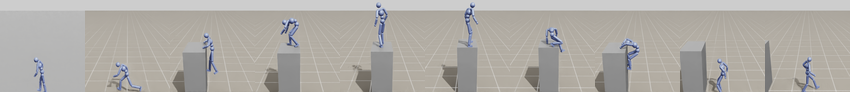
\includegraphics[width=0.92\textwidth]{figures/dare_climb_10.png}\\[-1pt]
{\footnotesize (a) Climb}\\[2pt]
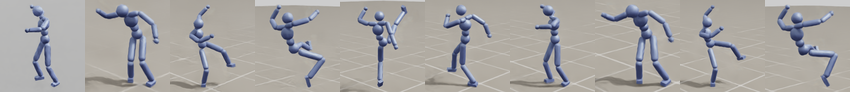
\includegraphics[width=0.92\textwidth]{figures/dare_spinkick_10.png}\\[-1pt]
{\footnotesize (b) Spin Kick}\\[2pt]
\begin{tabular}{@{}c@{\hspace{4pt}}c@{}}
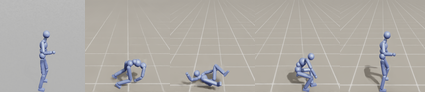
\includegraphics[width=0.47\textwidth]{figures/dare_roll_5.png} &
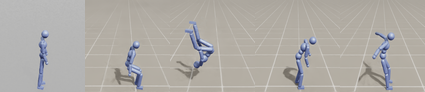
\includegraphics[width=0.47\textwidth]{figures/dare_backflip_5.png}\\[-1pt]
{\footnotesize (c) Roll} & {\footnotesize (d) Backflip}\\[2pt]
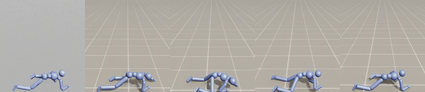
\includegraphics[width=0.47\textwidth]{figures/dare_crawl_5.png} &
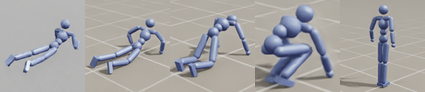
\includegraphics[width=0.47\textwidth]{figures/dare_getup_5.png}\\[-1pt]
{\footnotesize (e) Crawl} & {\footnotesize (f) Get-Up}
\end{tabular}
\end{tabular}
\caption{DARE policies executing the six skills in Isaac Lab using the shared
configuration in Table~\ref{tab:config}. Frames are uniformly sampled from
each rollout and rendered from a fixed front-view camera. Climb and Spin Kick
are shown with ten frames, and the remaining skills with five.}
\label{fig:snapshots}
\end{figure*}

\begin{figure*}[t]
\centering
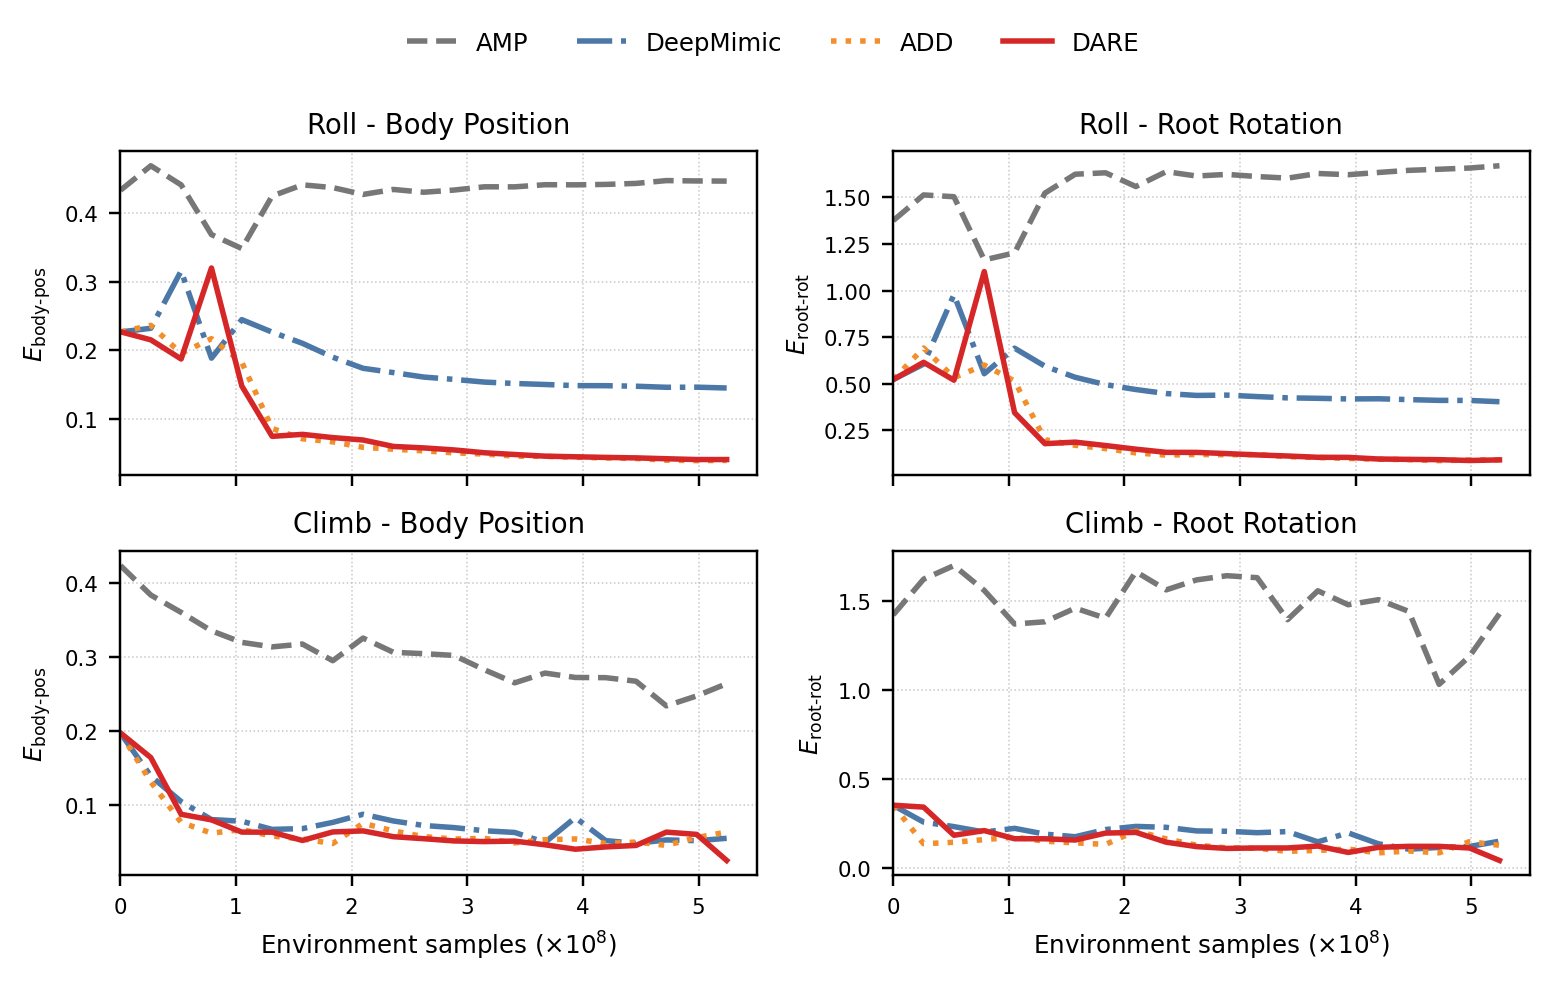
\includegraphics[width=0.82\textwidth]{figures/fig_learning_curves.png}
\caption{Learning curves for Roll and Climb under the matched training
budget. Curves show the mean over five independent seeds. The four panels
report body-position and root-rotation errors versus environment samples,
representing articulated translational fidelity and global orientation
tracking, respectively. Lower is better.}
\label{fig:learning}
\end{figure*}

\subsection{Experimental Setup}
\label{sec:setup}
All methods are evaluated using the same $28$-DoF, $15$-body humanoid
model adopted in prior physics-based motion-imitation studies, simulated in
Isaac Lab at $120\,\mathrm{Hz}$ with actions applied at $30\,\mathrm{Hz}$
through PD joint-position control
\cite{mittal2023isaaclab,makoviychuk2021isaacgym}. All four methods share
the same environment, training budget, motion clips, random-phase
initialization, and evaluation protocol. Each policy is trained for
$2000$ iterations of $8192$ environments $\times$ $32$ steps
($5.24\times10^8$ samples) with five independent seeds, and is evaluated
on $4096$ episodes per seed from randomly sampled reference phases. Actor
and value networks are two-layer MLPs ($1024$, $512$), and the PPO
settings (clip $0.2$, GAE $0.95$, $\gamma=0.99$, SGD with momentum $0.9$)
are fixed across methods. DARE additionally uses the normalizer and
one-shot logit calibration specified in Table~\ref{tab:config}.

The benchmark contains six skills with substantially different motion
durations, contact patterns, and dynamical characteristics: Roll, Climb,
Backflip, Crawl, Get-Up, and Spin Kick. Training termination follows each
method's environment configuration (pose termination is enabled for
DeepMimic, ADD, and DARE and disabled for AMP). The evaluation harness
accumulates each metric over the executed reference-aligned steps and uses
the same aggregation rule for every method; terminated trajectories are not
padded with synthetic states. Final policies reach essentially the full
prescribed evaluation horizon, so early termination has negligible effect
on the reported averages.

We use six complementary measures. The four geometric measures quantify
frame-wise imitation fidelity, whereas foot progress and lateral drift capture
trajectory-level behavior that is not summarized by instantaneous pose errors.
Four describe geometric tracking at two spatial levels: root position and
root rotation measure global translation and orientation, while body position
and body rotation measure articulated-body tracking. For an evaluation
trajectory with $B$ bodies, where $r,p_b$ and $q,q_b$ denote simulated root,
body positions and orientations and hats denote reference values, these
quantities are
\begingroup
\setlength{\abovedisplayskip}{0pt plus 1pt minus 1pt}
\setlength{\belowdisplayskip}{0pt plus 1pt minus 1pt}
\begin{align}
 E_{\mathrm{root\text{-}pos}}&=\lVert\hat r-r\rVert_2,
 \quad
 E_{\mathrm{root\text{-}rot}}=\angle(q,\hat q), \notag\\
 E_{\mathrm{body\text{-}pos}}&=\frac{1}{B}\sum_{b=1}^{B}
   \left\lVert(\hat p_b-\hat r)-(p_b-r)\right\rVert_2, \notag\\
 E_{\mathrm{body\text{-}rot}}&=\frac{1}{B}\sum_{b=1}^{B}\angle(q_b,\hat q_b).
\label{eq:geometric_metrics}
\end{align}
\endgroup
where $\angle(\cdot,\cdot)$ is the shortest angle between normalized
quaternions. Geometric quantities are evaluated at each reference-aligned
timestep and then averaged over executed timesteps and episodes; the two
behavior measures are computed per trajectory and then averaged over episodes.
The remaining two measures describe motion-level behavior.
Let $\Delta r$ and $\Delta\hat r$ be the simulated and reference root
displacements over the evaluated trajectory, and let
$\Delta p_j,\Delta\hat p_j$ be the corresponding displacements of foot $j$.
The reference-projected progress and transverse drift are
\begin{align}
 \rho_{\mathrm{foot}}&=\min_j
 \frac{\Delta p_j^{\top}\Delta\hat p_j}
      {\lVert\Delta\hat p_j\rVert_2^2}, \notag\\
 \rho_r&=\frac{\Delta r^{\top}\Delta\hat r}
                 {\lVert\Delta\hat r\rVert_2^2}, \notag\\
 E_{\mathrm{lat}}&=
 \frac{\left\lVert\Delta r-
 \rho_r\Delta\hat r\right\rVert_2}{\lVert\Delta\hat r\rVert_2}.
\label{eq:behavior_metrics}
\end{align}
Foot progress is ideal at one, while lateral drift is minimized at zero.
All six quantities are averaged over the evaluation trajectories; lower is
better except for foot progress, whose target value is one.

\subsection{Cross-Motion Tracking}
Table~\ref{tab:main} asks whether one configuration can serve skills whose
contacts, horizons, and velocity profiles differ, and
Fig.~\ref{fig:snapshots} shows the resulting controllers executing the six
skills in Isaac Lab. With one configuration shared across all six skills,
DARE achieves the best macro-average on all six measures. It yields the
lowest root- and body-level position and rotation errors, the
foot-progress ratio closest to one, and the lowest lateral drift.
Relative to the strongest baseline for each measure, root-position error,
root-rotation error, and lateral drift are reduced by approximately
$25\%$, $21\%$, and $38\%$.

\subsection{Learning Dynamics}
\label{sec:learning}
Figure~\ref{fig:learning} compares the five-seed mean body-position and
root-rotation errors against environment samples for Roll and Climb, which
provide contrasting motion durations and contact structures. Across both,
the DARE curves converge to lower errors under the same sample budget,
complementing the final-checkpoint comparison in Table~\ref{tab:main}.


\subsection{Component Analysis}
\label{sec:ablation}
We isolate the two components that define DARE's critic: layer-wise
spectral normalization and one-shot score calibration. This gives a
$2\times2$ comparison while keeping the differential input,
binary objective, replay procedure, PPO budget, and evaluation protocol
fixed. The study covers eight motions---Roll, Climb, Backflip, Crawl,
Get-Up, Spin Kick, Push Box, and Sit on Sofa---with three independent seeds
for every configuration. Entries are macro-averaged over the eight motions
for each seed and then summarized as a mean $\pm$ standard deviation; cells
whose measurements are still pending are marked in red.

\begin{table}[h]
\caption{Component analysis over eight motions. SN and Cal. denote
layer-wise spectral normalization and one-shot calibration. Lower is
better; red entries are pending measurements.}
\label{tab:ablation}
\centering
\scriptsize
\setlength{\tabcolsep}{1.5pt}
\begin{tabular}{lccrrrrr}
\toprule
Method & SN & Cal. & R.Pos. $\downarrow$ & B.Pos. $\downarrow$
 & R.Rot. $\downarrow$ & B.Rot. $\downarrow$ & DoF Vel. $\downarrow$ \\
\midrule
DARE & $\checkmark$ & $\checkmark$
 & \todo{--} & \todo{--} & \todo{--} & \todo{--} & \todo{--} \\
w/o SN & $\times$ & $\checkmark$
 & \todo{--} & \todo{--} & \todo{--} & \todo{--} & \todo{--} \\
w/o Cal. & $\checkmark$ & $\times$
 & \todo{--} & \todo{--} & \todo{--} & \todo{--} & \todo{--} \\
Base & $\times$ & $\times$
 & \todo{--} & \todo{--} & \todo{--} & \todo{--} & \todo{--} \\
\bottomrule
\end{tabular}
\end{table}

\FloatBarrier
\section{Conclusion}
Manual tracking rewards turn the aggregation of heterogeneous imitation
objectives into per-motion engineering. Learned differential rewards
remove the component-wise weights, but regularization can still couple the
critic's geometric sensitivity to the score range seen by the policy.
DARE treats these as separate design quantities: layer-wise spectral
normalization constrains the critic's sensitivity, and one closed-form
calibration sets the score scale without a motion-specific coefficient.
The score change relative to the unique zero differential is bounded by
the normalized residual, and the critic is then rescaled once, in closed
form, to set its operating scale relative to the response width of the
reward transform. Across the six skills, DARE attains the
lowest macro-average for all four geometric errors, the foot-progress
ratio closest to one, and the smallest lateral drift in
Table~\ref{tab:main}. The formulation also provides a direct path toward
multi-clip training and other morphologies, where additional objectives
can be incorporated directly into the differential.

\FloatBarrier
\footnotesize
\begin{thebibliography}{99}
\setlength{\itemsep}{0pt}
\bibitem{peng2018deepmimic}
X.~B. Peng, P.~Abbeel, S.~Levine, and M.~van~de~Panne, ``DeepMimic:
Example-guided deep reinforcement learning of physics-based character
skills,'' \emph{ACM Trans. Graph.}, vol.~37, no.~4, 2018.
\bibitem{luo2023phc}
Z.~Luo, J.~Cao, A.~W. Winkler, K.~Kitani, and W.~Xu, ``Perpetual humanoid
control for real-time simulated avatars,'' in \emph{Proc. ICCV}, 2023.
\bibitem{tessler2023maskedmimic}
C.~Tessler, Y.~Guo, O.~Nabati, G.~Chechik, and X.~B. Peng, ``MaskedMimic:
Unified physics-based character control through masked motion inpainting,''
\emph{ACM Trans. Graph.}, 2024.
\bibitem{ho2016gail}
J.~Ho and S.~Ermon, ``Generative adversarial imitation learning,'' in
\emph{Advances in Neural Information Processing Systems}, 2016.
\bibitem{peng2021amp}
X.~B. Peng, Z.~Ma, P.~Abbeel, S.~Levine, and A.~Kanazawa, ``AMP: Adversarial
motion priors for stylized physics-based character control,'' \emph{ACM Trans.
Graph.}, vol.~40, no.~4, 2021.
\bibitem{zhang2025add}
Z.~Zhang, S.~Bashkirov, D.~Yang, Y.~Shi, M.~Taylor, and X.~B. Peng,
``Physics-based motion imitation with adversarial differential
discriminators,'' in \emph{SIGGRAPH Asia Conf. Papers}, 2025.
\bibitem{gulrajani2017improved}
I.~Gulrajani, F.~Ahmed, M.~Arjovsky, V.~Dumoulin, and A.~Courville,
``Improved training of Wasserstein GANs,'' in \emph{Advances in Neural
Information Processing Systems}, 2017.
\bibitem{miyato2018spectral}
T.~Miyato, T.~Kataoka, M.~Koyama, and Y.~Yoshida, ``Spectral normalization
for generative adversarial networks,'' in \emph{Proc. ICLR}, 2018.
\bibitem{karras2020ada}
T.~Karras \textit{et al.}, ``Training generative adversarial networks with
limited data,'' in \emph{Advances in Neural Information Processing
Systems}, 2020.
\bibitem{sener2018multitask}
O.~Sener and V.~Koltun, ``Multi-task learning as multi-objective
optimization,'' in \emph{Advances in Neural Information Processing Systems},
2018.
\bibitem{kendall2018multi}
A.~Kendall, Y.~Gal, and R.~Cipolla, ``Multi-task learning using uncertainty
to weigh losses for scene geometry and semantics,'' in \emph{Proc. CVPR},
2018.
\bibitem{schulman2017ppo}
J.~Schulman, F.~Wolski, P.~Dhariwal, A.~Radford, and O.~Klimov, ``Proximal
policy optimization algorithms,'' arXiv:1707.06347, 2017.
\bibitem{schulman2016gae}
J.~Schulman, P.~Moritz, S.~Levine, M.~Jordan, and P.~Abbeel,
``High-dimensional continuous control using generalized advantage
estimation,'' in \emph{Proc. ICLR}, 2016.
\bibitem{makoviychuk2021isaacgym}
V.~Makoviychuk \textit{et al.}, ``Isaac Gym: High performance GPU-based
physics simulation for robot learning,'' in \emph{Proc. NeurIPS Datasets
and Benchmarks}, 2021.
\bibitem{mittal2023isaaclab}
M.~Mittal \textit{et al.}, ``Orbit: A unified simulation framework for
interactive robot learning environments,'' \emph{IEEE Robot. Autom.
Lett.}, vol.~8, no.~6, 2023.
\end{thebibliography}
\end{document}